\documentclass{sintefbeamer}

% packages, font, color, and newcommands
\usepackage{amsfonts, amsmath, oldgerm, lmodern, bm}
% \usepackage[font={footnotesize}]{caption}
\usepackage{natbib}
\usepackage{url}
\usepackage{tikz}
\usepackage{amssymb}
\usepackage{amsmath}
\usepackage{amsthm}
\usepackage{mathrsfs}
\usepackage{empheq}
\usepackage{mdframed}
\usepackage{bm}
\usepackage{animate}
\usepackage{xcolor,colortbl}
\usepackage{graphicx}
\bibliographystyle{apalike}
\usefonttheme{serif}
\usetikzlibrary{calc}

\title{Theoretical prediction of the Reynolds stress in low inertial buoyant emulsion.}
\subtitle{Based on the nearest particle statistic}
\author{\href{http://basilisk.fr/sandbox/fintzin/Rising-Suspenion/RS.c}{\underline{N. Fintzi}\footnote{IFP \'Energies Nouvelles, France}$^{,2}$}, JL. Pierson$^1$ and S. Popinet\footnote{Sorbonne Universit\'e, France}}
% \date{Created on May 22, 2022}

\titlebackground{image/3D/P_PHI_5.png}

% document body
\addtobeamertemplate{navigation symbols}{}{%
    \usebeamerfont{footline}%
    \usebeamercolor[fg]{footline}%
    % \hspace{1em}%
    % \vspace{1em}%
    \insertframenumber/\inserttotalframenumber
}
\usepackage{stmaryrd}
\newcommand{\Jump}[1]{\llbracket #1 \rrbracket \cdot \textbf{n} }

\newcommand{\size}{0.22\textwidth}
\newcommand{\avg}[1]{\left<#1\right>}
%\newcommand{\condavg}[1]{\left<#1 | \mathscr{C}_1\right>}
\newcommand{\Exp}[1]{\overline{\overline{#1}}}
\newcommand{\davg}[1]{\left<#1\right>_d}
\newcommand{\avgcond}[1]{\overline{#1}}
% \renewcommand{\avgcond}[1]{\left{#1}}
\newcommand{\kavg}[1]{\avgcond{#1}^k}
\newcommand{\cavg}[1]{\avgcond{#1}^c}
\newcommand{\Tavg}[1]{\avgcond{#1}^T}
\newcommand{\Xavg}[1]{\avgcond{#1}^X}
\newcommand{\TXavg}[1]{\Tavg{\Xavg{#1}}}
\newcommand{\Iavg}[1]{\left<#1\right>_I}
\newcommand{\pavg}[1]{n \left<#1\right>}
\newcommand{\pnavg}[1]{\left<#1\right>}
\newcommand{\nstavg}[1]{\overline{#1}^{nst}}
\newcommand{\condavg}[2]{\overline{#1}^{#2}}
\newcommand{\nstrelavg}[1]{\overline{#1}_{nst}^{rel}}
\newcommand{\mavg}[1]{\left<#1\right>_m}
\newcommand{\gavg}[2][\gamma]{\left<#2\right>_{#1}}
\newcommand{\partials}[1]{\partial_{i_1}\partial_{i_2}\ldots\partial{i_{#1}}}
\newcommand{\partialp}[2]{ \prod_{m=#1}^{#2} \partial_{i_m}}
\newcommand{\hatpartialp}[2]{ \prod_{m=#1}^{#2} \hat{\partial}_{j_m}}
\newcommand{\hatpartialpi}[2]{ \prod_{m=#1}^{#2} \hat{\partial}_{i_m}}
\newcommand{\pri}[2]{ \prod_{m=#1}^{#2} r_{i_m}}
\newcommand{\prj}[2]{ \prod_{m=#1}^{#2} r_{j_m}}
\newcommand{\nablab}{\bm{\nabla}}
\newcommand{\nablabh}{\hat{\bm{\nabla}}}
\newcommand{\ddt}{\frac{d}{d t}}
\newcommand{\pddt}{\partial_t}
% \newcommand{\pddt}{\partial t \;}

\newcommand{\CC}{\mathscr{C}}
\newcommand{\PP}{\mathscr{P}}
\newcommand{\tb}[1]{\color{blue}#1\color{black}}
% \renewcommand{\tb}[1]{}

% \renewcommand{\ref}[1]{\autoref{#1}}
\renewcommand{\size}[1]{0.3\textwidth}
\newcommand{\expo}[1]{\frac{(-1)^n}{n!} \partialp{1}{n} \pavg{\int_{\Omega_\alpha} \pri{1}{n}#1 d\Omega}}

\usepackage{amsmath}


\begin{document}
\maketitle

\begin{frame}
  \frametitle{The ensemble average fluid phase Reynolds stress}
  \begin{equation*}
    \avg{\chi_k \textbf{u}'_k\textbf{u}'_k}(\textbf{x},t)
    % = \int \nstavg{\chi_k \textbf{u}_k^0\textbf{u}_k^0}  P_{nst}(\textbf{x},t,\textbf{r}) d\textbf{r}
    % - \phi_k \textbf{u}_k\textbf{u}_k
    = \int  \chi_k \textbf{u}^0_k\textbf{u}^0_k(\textbf{x},t,\CC) P(\CC)d\CC 
    - \phi_k \textbf{u}_k\textbf{u}_k
\end{equation*}

\begin{itemize}
  \item $\textbf{u}_k^0$ local instantaneous velocity fields;
  \item $\chi_k$ phase indicator function;
  \item $\textbf{u}_k$ phase averaged velocity fields;
  \item $\phi_k$ volume fraction;
  \item $\CC$ a configuration of the flow;
  \item $P(\CC)$ probability density of $\CC$.
\end{itemize}


\underline{How to find a theoretical expression ??? }
\end{frame}
\begin{frame}
  \frametitle{L.Van Wijngaarden approach for potential flow.}

The potential flow solution of an isolated translating spheres is :
\begin{equation*}
  \textbf{u}'_\text{potential}
  = \frac{a^3 \textbf{U}}{2}\left(\frac{1}{r^3} - \frac{3 \textbf{xx}}{r^5}\right).
  \text{    for    }r>a
\end{equation*}

Therefore, the Reynolds stress approximation in homogeneous dilute suspension of spherical bubbles can be written Wijngaarden(1976): 
  \begin{align*}
    \avg{\chi_k \textbf{u}'_k\textbf{u}'_k}(\textbf{x},t)
    &\approx \int \textbf{u}'_\text{potential}\textbf{u}'_\text{potential}  P_1(\textbf{x},t,\textbf{r}) d\textbf{r}
    - \phi_k \textbf{u}_k\textbf{u}_k\\
    &= \phi_k \left(\frac{3}{20} U^2\textbf{I} + \frac{1}{20}\textbf{UU} \right)
    % = \int  \chi_k \textbf{u}^0_k\textbf{u}^0_k(\textbf{x},t,\CC) P(\CC)d\CC 
    % - \phi_k \textbf{u}_k\textbf{u}_k
\end{align*}


\begin{itemize}
  \item $P_1(\textbf{r}) = n_p$ is the probability of finding a particle center of mass at \textbf{r} which is equal to the number density $n_p$. 
  \item \textbf{U} is the drift velocity between phases. 
  \item $a$ is the radius of the spheres. 
  % \item This relation is valid for infinitely dilute suspension $n_p \to \infty$
  \item The integral converge because $\textbf{u}_\text{potential}  \sim r^{-3}$
\end{itemize}

\end{frame}

\begin{frame}
  \frametitle{Stokes flow around a translating spherical drop}
  The stokes flow solution of an isolated translating drop is :

  \begin{equation*}
    \textbf{u}_\text{stokes} 
    = \left(\frac{ \textbf{I}}{r} + \frac{\textbf{rr}}{r^3}\right)  \frac{1}{4}\left(\frac{3\lambda + 2}{\lambda +1}\right) a \textbf{U}
    - \left(-\frac{\textbf{I}}{r^3} + \frac{3 \textbf{rr} }{r^5}\right)  \frac{1}{4}\left(\frac{\lambda}{\lambda +1}\right) a^3 \textbf{U}
  \end{equation*}

  \begin{itemize}
    \item $\lambda$ is the viscosity ratio.
  \end{itemize}
  
  Let's apply Wijngaarden approach on this solution : 
  \begin{align*}
    \avg{\chi_k \textbf{u}'_k\textbf{u}'_k}(\textbf{x},t)
    &\approx \int \textbf{u}'_\text{stokes}\textbf{u}'_\text{stokes}  P_1(\textbf{x},t,\textbf{r}) d\textbf{r}
    - \phi_k \textbf{u}_k\textbf{u}_k
    =\infty 
  \end{align*}
  \underline{The integral diverges since $\textbf{u}_\text{stokes} \sim r^{-1}$.}

  $\to$ Indeed in an infinitely dilute situation in stokes regime the Reynolds stress is indeed infinite.

  $\to$ Consequently, we must use another method which consider a finite volume fraction $\phi$. 
\end{frame}

\begin{frame}
  \frametitle{The nearest particle statistics decomposition}
  \begin{multline*}
    \avg{\chi_k \textbf{u}'_k\textbf{u}'_k}(\textbf{x},t)
    = 
    \underbrace{\int (\nstavg{\chi_k \textbf{u}^0_k}  \nstavg{\chi_k \textbf{u}^0_k} / (\nstavg{\chi_k})  P_{nst}(\textbf{x},t,\textbf{r}) d\textbf{r} }_\text{PWFs}
    \\+\underbrace{\int \nstavg{\chi_k \textbf{v}_k^0\textbf{v}_k^0}  P_{nst}(\textbf{x},t,\textbf{r}) d\textbf{r}}_\text{WIA}
    - \phi_k \textbf{u}_k\textbf{u}_k
  \end{multline*}

\begin{itemize}
  \item $\textbf{v}_k^0  = \textbf{u}_k^0 - \nstavg{\chi_k \textbf{u}^0_k} / \nstavg{\chi_k}$ is the fluctuation of the local velocity relative to the nearest averaged value. 
  \item This relation is exact and require no assumption. 
\end{itemize}
\end{frame}

\begin{frame}
  \frametitle{Potential flow solution with this method}
  \begin{multline*}
    \avg{\chi_k \textbf{u}'_k\textbf{u}'_k}(\textbf{x},t)
    = 
    {\int \textbf{u}_\text{potential} \textbf{u}_\text{potential}  P_{nst}(\textbf{x},t,\textbf{r}) d\textbf{r} }
    - \phi_k \textbf{u}_k\textbf{u}_k\\
    = \phi_k \left(\frac{3}{20} U^2\textbf{I} + \frac{1}{20}\textbf{UU} \right)
    \Gamma_\text{inc}(-1,\phi)\phi^2 e^\phi
  \end{multline*}

  \begin{itemize}
    \item \textbf{Hypothesis 1} : We considered $\textbf{v}^0_k =0$ since all the wake are considered similar. 
    \item \textbf{Hypothesis 2} : We considered $\textbf{u}_\text{nst} = \textbf{u}_\text{potential}$ since all the wake are considered similar. 
    \item We consider $P_{nst}(\textbf{x},t,\textbf{r}) = n_p e^{-4\pi n_p(r^3-a)/3}$ which is true for homogeneous flows. 
    \item $\Gamma_\text{inc}(a,x) = \int_x^\infty t^{a-1} e^{-t} dt $ is the incomplete gamma  function. 
  \end{itemize}

  $\to$ Notice that $\Gamma_\text{inc}(-1,\phi)\phi^2 e^\phi \rightarrow 1$ when $\phi \rightarrow 0$. Therefore, we recover  Wijngaarden(1976) solution in dilute regime. 
\end{frame}

\begin{frame}
  \frametitle{Reconstruction of the velocity fields from DNS}
  \begin{figure}[h!]
    \centering
    \begin{tikzpicture}
        \node (img) at (0,0)  {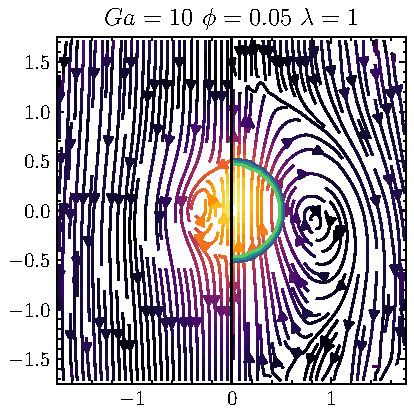
\includegraphics[height=0.25\textwidth]{image/HOMOGENEOUS/Stream/Stream_PHI_5_Ga_10_l_1.pdf}};
        \node (img) at (0.25\textwidth,0)  {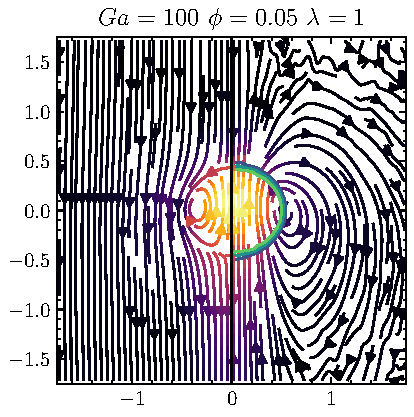
\includegraphics[height=0.25\textwidth]{image/HOMOGENEOUS/Stream/Stream_PHI_5_Ga_100_l_1.pdf}};
        \node (img) at (0.5\textwidth,0)  {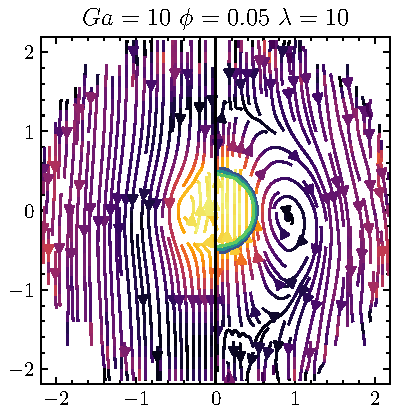
\includegraphics[height=0.25\textwidth]{image/HOMOGENEOUS/Stream/Stream_PHI_5_Ga_10_l_10.pdf}};
        \node (img) at (0.75\textwidth,0)  {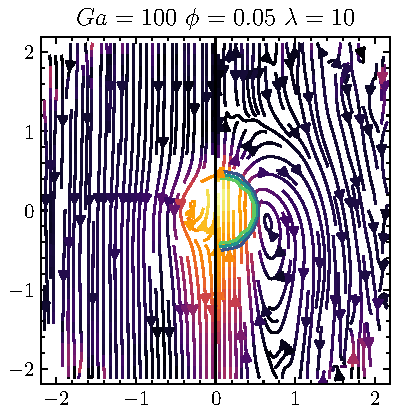
\includegraphics[height=0.25\textwidth]{image/HOMOGENEOUS/Stream/Stream_PHI_5_Ga_100_l_10.pdf}};
    \end{tikzpicture}
    \caption{Nearest particle averaged velocity $\nstavg{\textbf{u}}(\textbf{r})$ for  $\phi = 5\%$ and $20\%$.
    Green lines : contour plots of the nearest averaged indicator function $\nstavg{\chi_d}(\textbf{r})$ (it represent the mean shape of the particles)}
    \label{fig:Stream}
  \end{figure}
  
  \begin{itemize}
    \item Close from the drop ($r=\mathcal{O}(a)$) we can see that $\textbf{u}_\text{nst} \approx \textbf{u}_\text{stokes}$. 
  \end{itemize}
\end{frame}

\begin{frame}
  \frametitle{Nearest particle statistic solution for translating drops in stokes flow :}
  \begin{multline}
    \avg{\chi_k \textbf{u}'_k\textbf{u}'_k}(\textbf{x},t)
    = 
    {\int \textbf{u}_\text{stokes} \textbf{u}_\text{stokes}  P_{nst}(\textbf{x},t,\textbf{r}) d\textbf{r} }
    - \phi_k \textbf{u}_k\textbf{u}_k
    \\=
-\left({{-\left(9\,\Gamma\left(-1 , \,\phi\right)\,\lambda^2\,\phi
^{{{4}\over{3}}}\,e^{\phi}\right)+\ldots}\over{\left(120\,\lambda^2+240\,\lambda+
120\right)\,\phi^{{{1}\over{3}}}}}\right)
\textbf{e}_U\textbf{e}_U + \ldots
\end{multline}
\begin{itemize}
  \item $\textbf{e}_U$ is the units vector in the direction of the drift velocity. 
\end{itemize}

\end{frame}

\begin{frame}
  \frametitle{Comparison with DNS results }
  \begin{figure}[h!]
    \centering    
    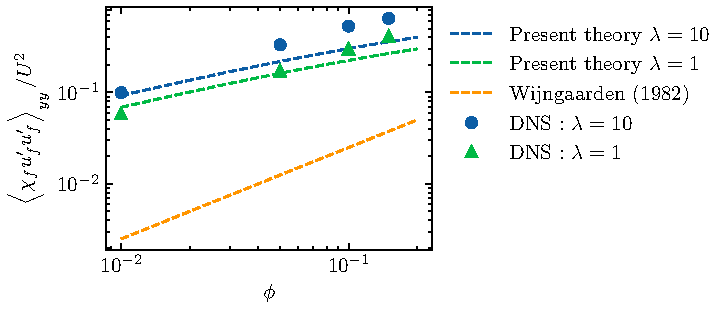
\includegraphics[height = 0.25\textwidth]{image/HOMOGENEOUS/fCA/Pseudo_turbe.pdf}
    \caption{
       Dimensionless \textbf{fluid phase pseudo turbulent kinetic energy} : $K_c \avg{\chi_k \textbf{u}'_k\textbf{u}'_k} : \textbf{I} \frac{1}{2}$ in terms of the volume fraction $\phi$ for two viscosity ratio $\lambda =1,10$ and $Re \approx 1$ DNS. 
    }
    \label{fig:Cp}
\end{figure}  
\begin{itemize}
  \item The tendency in terms of $\phi$ and $\lambda$ are right.  
  \item Quantitative agreement at $\phi \ll 1$ and not at $\phi <1$ because of the interactions.  
  \item The present theory solution indeed diverge in $\phi \to 0$ 
\end{itemize}
\end{frame}

\begin{frame}
  \frametitle{Comparison with DNS results }
  \begin{figure}[h!]
    \centering    
    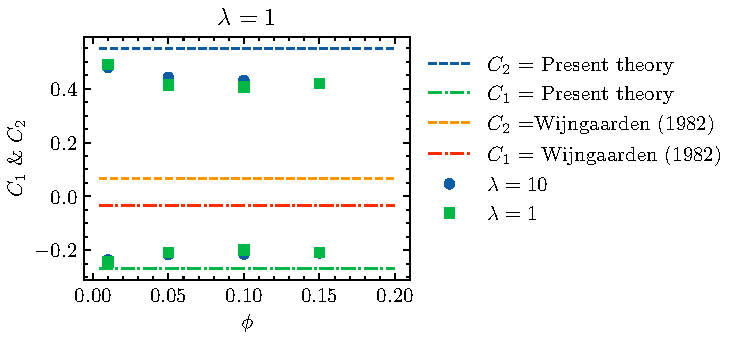
\includegraphics[height = 0.25\textwidth]{image/HOMOGENEOUS/fCA/Pseudo_turbe_coef.pdf}
    \caption{
       Coefficient of the Reynolds stress tensor in terms of the volume fraction $\phi$ for two viscosity ratio $\lambda =1,10$ and $Re \approx 1$ DNS. 
    }
    \label{fig:Cp}
\end{figure}  
Where we have defined :
\begin{equation*}
  \avg{\chi_1\textbf{u}_1'\textbf{u}_1'}
  = k^*_1 \left[
      \textbf{U}
      \textbf{U}
      (C_1  - C_2 )
      + \textbf{I} 
      (\textbf{U}\cdot\textbf{U})  (C_1+2/3) 
  \right]
\end{equation*}
\end{frame}


\begin{frame}
  \frametitle{Particle phase kinetic energy}
  Assuming \textbf{force free} particle in stokes flow one can also derive the Reynolds stress from nearest particle statistic. 
  \begin{figure}[h!]
    \centering    
    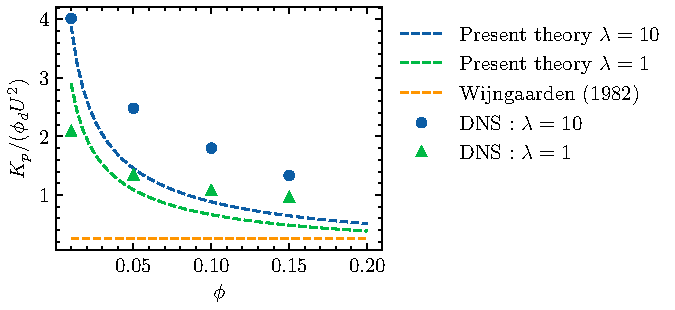
\includegraphics[height = 0.25\textwidth]{image/HOMOGENEOUS/fCA/Pseudo_turbeP.pdf}
    \caption{
       Dimensionless \textbf{granular temperature} in terms of the volume fraction $\phi$ for two viscosity ratio $\lambda =1,10$ and $Re \approx 1$ DNS. 
    }
    \label{fig:Cp}
\end{figure}  
\begin{itemize}
  \item The tendency in terms of $\phi$ and $\lambda$ are right.  
  \item Quantitative agreement at $\phi \ll 1$.  
\end{itemize}


\end{frame}
\end{document}
